%%%%%%%%%%%%%%%%%%%%%%%%%%%%%%%%%%%%%%%%%%%%%%%%%%%%%%%%%%%%%

\documentclass[a4paper,12pt]{scrartcl} %This is a special class provided by the KOMA script, which does a lot of adjustments to adapt the standard LaTeX classes to european habits, change to [a4paper,12pt,twoside] for doublesided layout


%########################### Preferences #################################


% ******** vmargin settings *********
\usepackage{vmargin} %This give you full control over the used page arae, it maybe not the idea od Latex to do so, but I wanted to reduce to amount of white space on the page
\setpapersize{A4}
\setmargins{3.5cm}%			%linker Rand, left edge
			{1.5cm}%     %oberer Rand, top edge
           {14.7cm}%		%Textbreite, text width
           {23.42cm}%   %Texthoehe, text hight
           {14pt}%			%Kopfzeilenhöhe, header hight
           {1cm}%   	  %Kopfzeilenabstand, header distance
           {0pt}%				%Fußzeilenhoehe footer hight
           {2cm}%    	  %Fusszeilenabstand, footer distance         

% ********* Font definiton ************
\usepackage{t1enc} % as usual{\Large\bf\sf \begin{tabular}{cc}Jessica Larsson &\textit{<jesbe726>}\\ Birgit Saalfeld &\textit{<birsa476>}\end{tabular}}
\usepackage[latin1]{inputenc} % as usual
\usepackage{times}		
%\usepackage{mathptmx}  	%mathematical fonts for use with times, I encountered some problems using this package togather with pdftex, which I was not able to resolve

% ********* Graphics definition *******
\usepackage[pdftex]{graphicx} % required to import graphic files
\usepackage{color} %allows to mark some entries in the tables with color
\usepackage{eso-pic} % these two are required to add the little picture on top of every page
\usepackage{everyshi} % these two are required to add the little picture on top of every page
\renewcommand{\floatpagefraction}{0.7} %default:0.5 allows two big pictures on one page

%********** Enybeling Hyperlinks *******
\usepackage[pdfborder=000,pdftex=true]{hyperref}% this enables jumping from a reference and table of content in the pdf file to its target

% ********* Table layout **************
\usepackage{booktabs}	  	%design of table, has an excellent documentation
%\usepackage{lscape}			%use this if you want to rotate the table together with the lines around the table

% ********* Caption Layout ************
\usepackage{ccaption} % allows special formating of the captions
\captionnamefont{\bf\footnotesize\sffamily} % defines the font of the caption name (e.g. Figure: or Table:)
\captiontitlefont{\footnotesize\sffamily} % defines the font of the caption text (same as above, but not bold)
\setlength{\abovecaptionskip}{0mm} %lowers the distace of captions to the figure


% ********* Header and Footer **********
% This is something to play with forever. I use here the advanced settings of the KOMA script

\usepackage{scrpage2} %header and footer using the options for the KOMA script
\renewcommand{\headfont}{\footnotesize\sffamily} % font for the header
\renewcommand{\pnumfont}{\footnotesize\sffamily} % font for the pagenumbers

%the following lines define the pagestyle for the main document
\defpagestyle{cb}{%
(\textwidth,0pt)% sets the border line above the header
{\pagemark\hfill\headmark\hfill}% doublesided, left page
{\hfill\headmark\hfill\pagemark}% doublesided, right page
{\hfill\headmark\hfill\pagemark}%  onesided
(\textwidth,1pt)}% sets the border line below the header
%
{(\textwidth,1pt)% sets the border line above the footer
{{\it Federation Confidential}\hfill Chief O'Brian}% doublesided, left page
{Chief O'Brian\hfill{\it Federation Confidential}}% doublesided, right page
{Larsson, Saalfeld\hfill{\it OMR }} % one sided printing
(\textwidth,0pt)% sets the border line below the footer
}

%this defines the page style for the first pages: all empty
\renewpagestyle{plain}%
	{(\textwidth,0pt)%
		{\hfill}{\hfill}{\hfill}%
	(\textwidth,0pt)}%
	{(\textwidth,0pt)%	
		{\hfill}{\hfill}{\hfill}%
	(\textwidth,0pt)}

%********** Footnotes **********
\renewcommand{\footnoterule}{\rule{5cm}{0.2mm} \vspace{0.3cm}} %increases the distance of footnotes from the text
\deffootnote[1em]{1em}{1em}{\textsuperscript{\normalfont\thefootnotemark}} %some moe formattion on footnotes

%################ End Preferences, Begin Document #####################

\title{OMR}
\pagestyle{plain} % on headers or footers on the first page

\setlength{\parindent}{0mm}
\setlength{\parskip}{12pt}

\usepackage{paralist}
%\usepackage{subfigure}
\usepackage{caption}
\usepackage{subcaption}
%\usepackage{biblatex}
\usepackage{rotating}




\begin{document}

\begin{center}

\begin{figure}[th]
    \centering
		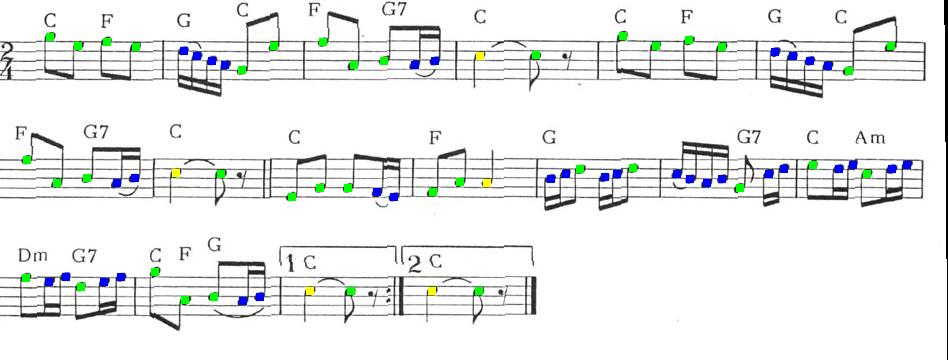
\includegraphics[width=\textwidth]{im1s_compare.jpg}
		\label{fig:logo}
\end{figure}

\vspace{2cm}

% There might be better solutions for the title page, giving all distances and sizes manually was simply the easiest solution

{\Huge\bf\sf Optical Music Recognition}

\vspace{.5cm}

{\Huge\bf\sf Project Assignment}

\vspace{.5cm}

{\large\bf\sf for the course 2013/ht2 \\ TNM034 Advanced Image Processing }

\vspace{2cm}

{\Large\bf\sf \begin{tabular}{cc}Jessica Larsson &\textit{<jesbe726>}\\ Birgit Saalfeld &\textit{<birsa476>}\end{tabular}}
\vspace{2cm}

{\Large\bf\sf Link\"{o}pings universitet, Norrk\"{o}ping\\ \today} %adds the current date

\vspace{\fill}

\end{center}



%\newpage

%\renewcommand{\abstractname}{Summary}

% fuer die ueberschrift, ohne nummer und ohne erwähnung im inhaltsverzeichnis
%\section*{Abstract}

% fuer die erwaehnung im inhaltsverzeichnis (ohne nummer)
%\addcontentsline{toc}{section}{Summary}




%This project report describes one method on how to program a simple OMR (optical music recognition) program. This is achieved by combining basic morphological operations and applying additional logic.  \\ \\
%In addition to the one method at hand, further approaches are discussed in the last chapter.  



\newpage


%%The following loads the picture on top of every page, the numbers in \put() define the position on the page:
%\AddToShipoutPicture{\setlength\unitlength{0.1mm}\put(604,2522){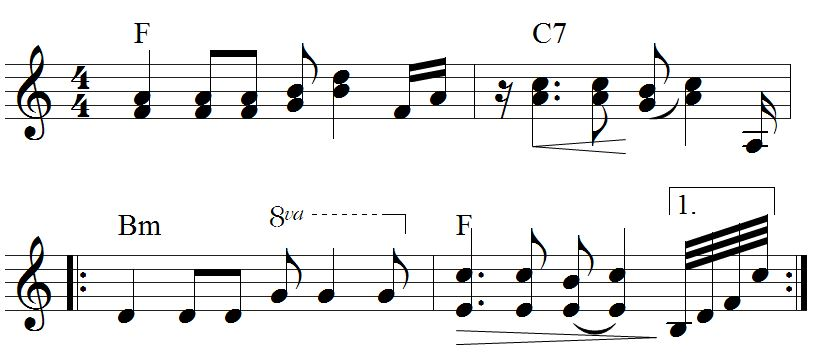
\includegraphics[width=1.5cm]{logo.jpg}}}

\pagestyle{cb} % now we want to have headers and footers


\tableofcontents
\newpage
\addcontentsline{toc}{section}{List of figures}
\listoffigures
\newpage


%##############################################################################
%##############################################################################
\section{Introduction}
%##############################################################################
%##############################################################################


%B warum ist notenerkennung wichtig, datenerhaltung, verfielfätltigung und so, organisatorische info eher später


Optical Music Recognition (OMR) is an extension of the Optical Character Recognition field and aims at translating music symbols from printed music sheets into digital format. The first documented approach of an OMR system was made by Pruslin in the 1960s. His program was able to detect primarily music notes, without being able to recognize other important characters such as pauses and G-clefs. Since then OMR has been an international research effort and has become quite advanced, but with challenges yet to be solved. \cite{bainb2001}  %?? WHICH CHALLENGES? 

This project, made in the course tnm034 - Advanced Image Processing at Link\"{o}pings University, aims at implementing an OMR system much like the one Pruslin had accomp
lished. Only a subset of all music symbols should be detected. The notes to be detected are quarter notes (crotchets) and eight notes (quavers) without taking any other characters and notes into account.

The program should take in an image normalized to the interval [0, 1] of captured sheet music and return as result a string of detected notes. The captured sheet music is either a scanned image or an image taken with a camera.  The pitures taken with camera can be for example distorted or not uniformly illuminated. Therefore preprocessing is necessary for some pictures.  


%?? MULTIPLE NOTES

This paper presents our implementation for Optical Music Recognition. The tool used to implement the OMR program is MATLAB, a powerful instrument that already has all the basic morphological operations implemented, reducing the amount of handwritten code. The focus will therefore be based on the combination of known techniques, like morpholgical operations instead of how explaining the theory behind those algorithms.

According to software engineering standards all komponents should be reusable. Therefore the main process of detecting the notes is decoupled from all prior steps. Preprocessing leads to a normalized input image. This image is binarized, complemented, cutted and rotated. If the input image is camera taken, more preprocessing steps are necessary to derive such a normalized picture, see figure~\ref{fig:flow}. During normalization, it is necessary to detect already the staff systems. With the staff information and the normalized image it is possible to create image variations. They will be used for detection of note heads and later on for detection of note values. Combining the obtained information it is possible to build the result string. 

In the following chapters the shown substeps of figure~\ref{fig:flow} will be described in more detail. The order of presentation is following the execution order. As written above the software is divided in two parts, so in this documentation every chapter deals with one of those parts.



\begin{figure}[htbp]
    \centering
    % links, unten rechts oben
		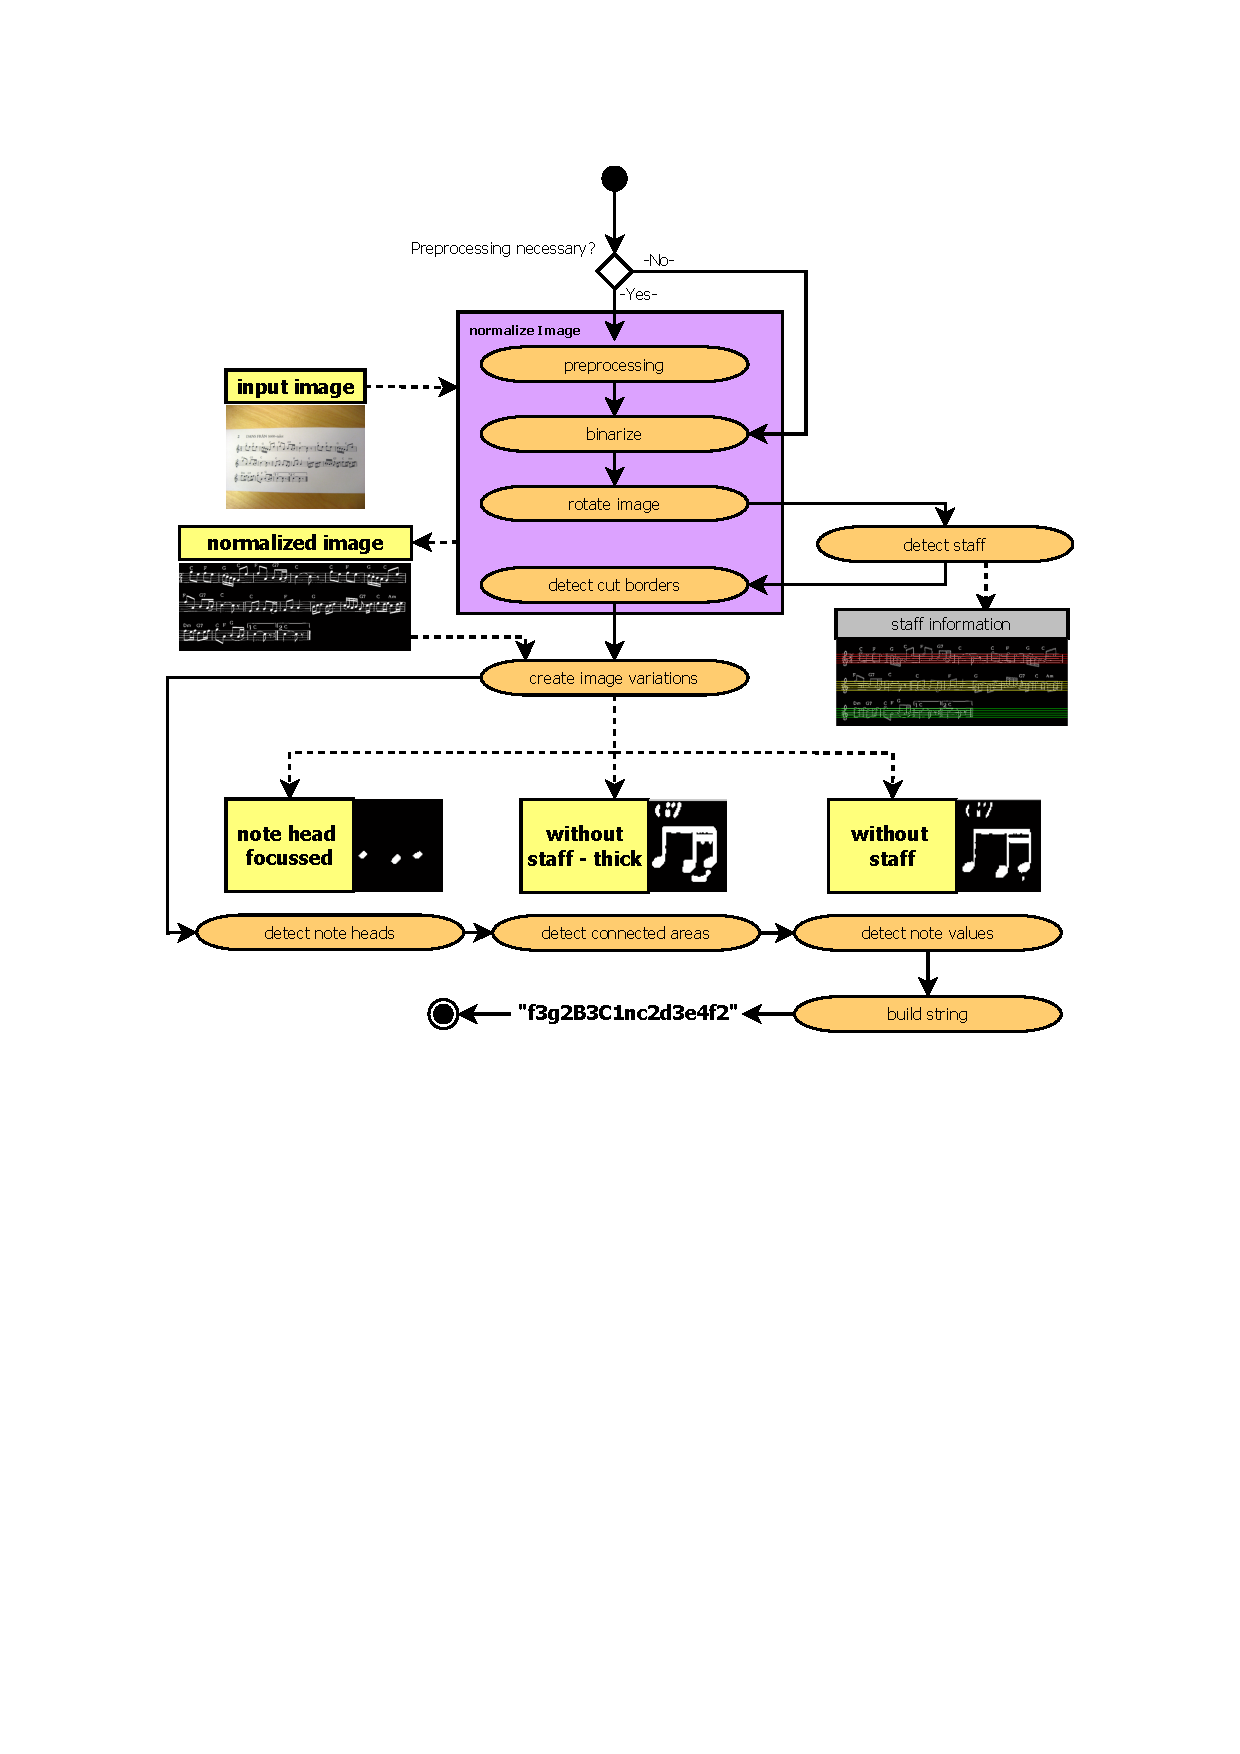
\includegraphics[width=\textwidth,trim=60  300 70 60, clip=true]{Diagram1.pdf}
		\caption {Simplified flow chart diagram \label{fig:flow}}
\end{figure}



%##############################################################################
%##############################################################################
\section{Normalize Images}
%##############################################################################
%##############################################################################
There are two types of input images that schould be evaluated with this software. One type are the scanned images without background information. More challenging are the pictures taken with camera. They introduces problems like distortion, out of focus, nonuniform illumitation or note detection disturbing background. Due to this reasons the software is devided into two parts. The main part note detection from scanned images. To extend this, the second part deals with preprocessing in order to convert the camera taken picture into a scanned liked picture. 

The software developed for the Advanced Image Processing course should be able to detect notes. To reduce the complexity of the task, limitations where introduced for this project: 

\begin{itemize}
\item All music sheets are computer generated and not handwritten 
\item Detect only quaters and crotches
\item Always assume G-clefs
\item The rotated image never exceeds $\pm 90$ degrees
\item All images taken with the camera are taken in front of the same background
\end{itemize}

%OMR is a complex task. All procedual programs consist out of many single steps. 



%#######################################
\subsection{Preprocessing}
%#######################################
Prepocessing is necessary for images with poor quality or pictures taken with a camera, because they can contain a lof of additional information, like backgound or they can be distorted. 

To handle the table in the background it is useful to focus on the blue channel of the image. If this channel differs a lot between the center and the sides of the input image there is with high probability a table on the image. With this blue channel information the table can get cutted away.

This code to undo the distortion is not implemented yet. One idea how to handle distortion is use of vandermonde matrix. This algorithms takes certain positions form the distorted images. Additionaly it needs the information where these points are located in the non distorted image. Then it calculates the transformation from one image into the other.

Furhtermore for following steps a global illumination has to be guaranteed. Global illumination can be reached by apply sliding maximum over the image, as shown in one of the course lectures.


For all scanned images the preprocessing should not change anything. 
%#######################################
\subsection{Rotate Image}
%#######################################

Another important step for normalization is the rotation of the picture. Therefore the rotation angle has to be determined. 

The rotation is achieved by first applying a Sobel operator to enhance all edges and then calculate the desired rotation degree, using the Hough transformation.
%?? wollen wir erklären, dass wir hough zweimal haben, global, lokal
From this hough transformation the 10 highest peaks are extracted and shown as blue lines in figure~\ref{fig:falsePositives}. There are even sometimes false positives. Those can be the borders of the sheet or ascending/descinding note rows, like the red marked in figure ~\ref{fig:falsePositives}.

\begin{figure}[htbp]
    \centering
    % links, unten rechts oben
		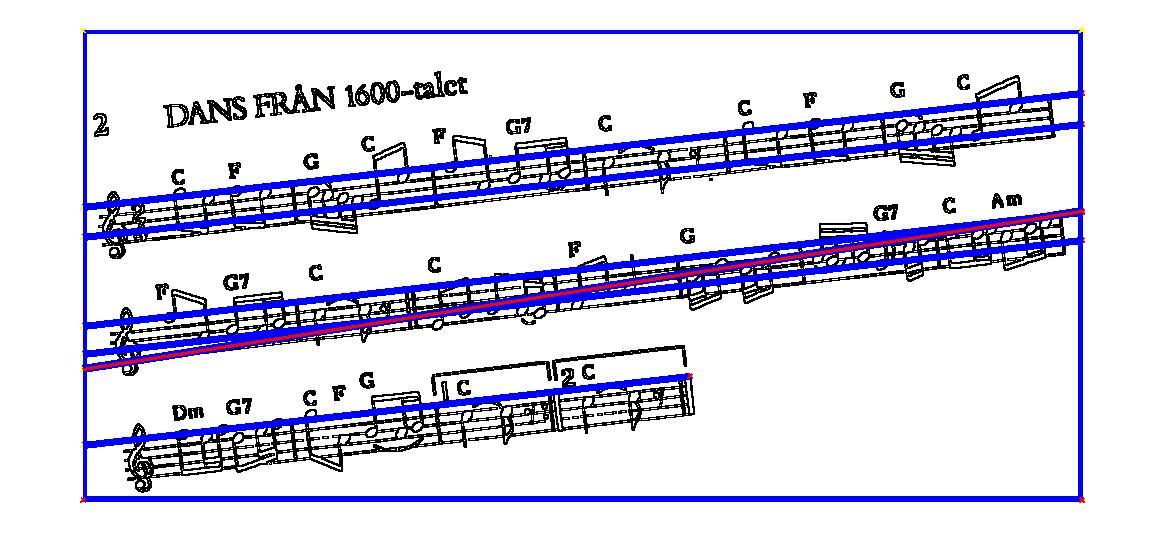
\includegraphics[width=0.85\textwidth]{detectRot1.jpg}
		\caption[10 Houghlines (blue) in detect rotation]{10 Houghlines (blue) in detect rotation, including false positives, like the red markes one\label{fig:falsePositives}}
\end{figure}

To avoid taking those false positives into account when calculating the rotation degree, only the 5 most similar lines are selected. The selection throws away the outliers, like vertical borders. The similarity of the lines is determined by comparing the absoulte value of their slopes. Removing the outlies ensures that no picture borders and no ascending/descending note rows are taken into account. From those remaining (random staff) lines the mean value is found for the optimal rotation, as shown in figure~\ref{fig:rotfind}.


\begin{figure}[htbp]
    \centering
    % links, unten rechts oben
		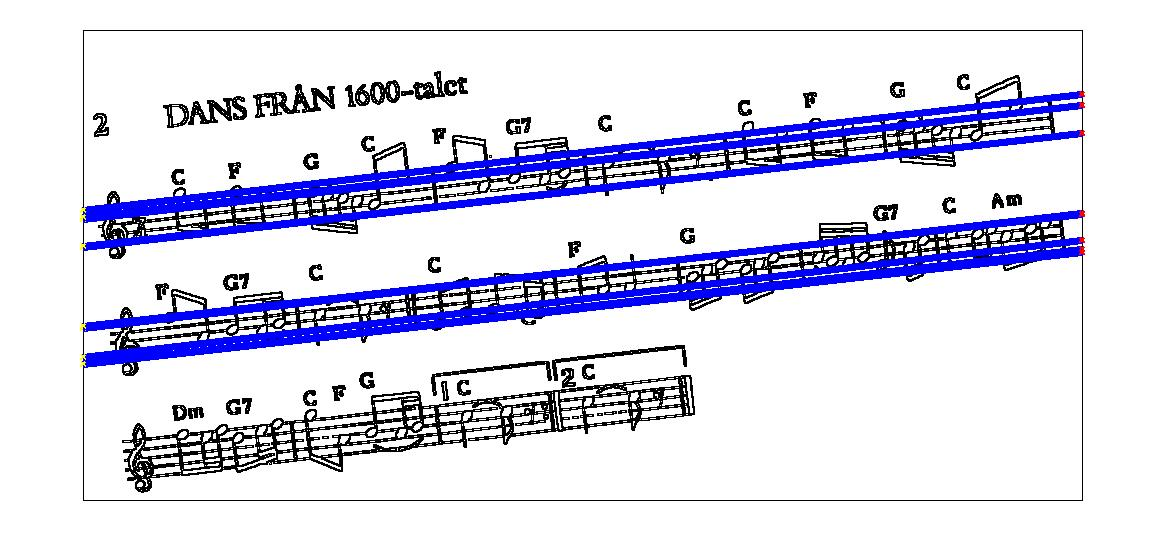
\includegraphics[width=0.85\textwidth]{detectRot2.jpg}
		\caption[5 remaining Houghlines (blue) in detect rotation]{5 remaining Houghlines (blue) in detect rotation\label{fig:rotfind}}
\end{figure}
 
%#######################################
\subsection{Detect staff system}
%#######################################
The staff systems are an important source of information. They yield information about where note heads are expected to be found and which pitch the note is. One staff system consists of five staff lines, all with roughly the same thickness (\textit{staffHeight}) and all with the same space between one another (\textit{staffSpace}). \cite{DalitzDPF08}



To detect the positions of the staff systems a horizontal projection is made on the complemeted binarized image, see figure~\ref{fig:staffBinComp}. 
In this rotated image the staff lines are horizontal. By counting the white pixels per row each staff line delivers a high amount of white pixels. So every high peak in the horizontal projection is with a high probability a staff line.


\begin{figure}[htbp]
    \centering
    % links, unten rechts oben
		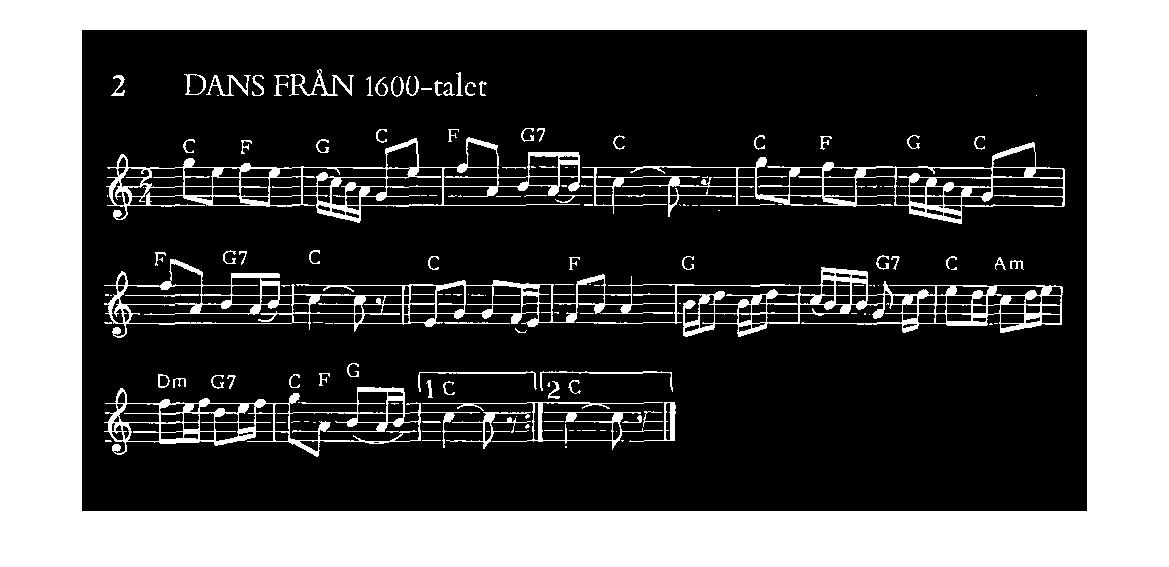
\includegraphics[width=0.85\textwidth]{staffBinComp.jpg}
		\caption{Binarized, complemented image\label{fig:staffBinComp}}
\end{figure}

Due to the \textit{staffHeight} is  thicker than one pixel in most cases it is necessary to concentrate this cluster of peaks to one peak. This can be achieved using a low pass filter, see figure~\ref{fig:staffHoriz}. After this filtering the peaks are lower, but then the peaks are more concentrated. 

\begin{figure}[htbp]
    \centering
    % links, unten rechts oben
		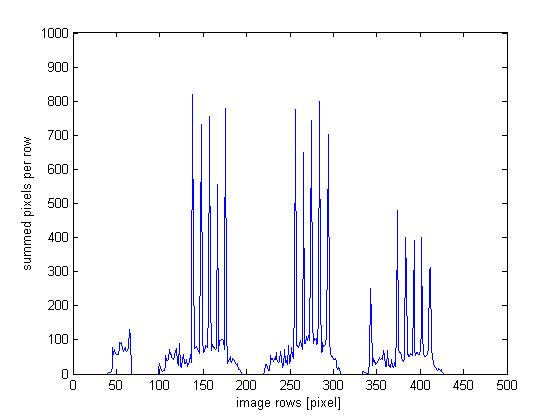
\includegraphics[width=0.48\textwidth]{staffHorizontal.jpg}
        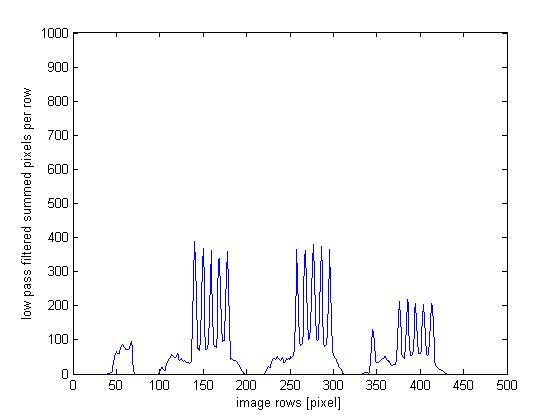
\includegraphics[width=0.48\textwidth]{staffHorizontalFiltered.jpg}
		\caption[Horizontal projections finding staff lines]{Horizontal projection unfiltered and filtered for finding staff lines\label{fig:staffHoriz}}
\end{figure}

The histogramm of figure~\ref{fig:staffHorizontalHist} shows the frequency of the normalized staff peak values. In the right half there are 10 peaks from the two long staff lines. In the middle part the short staff line can be seen. Everything below this values is not a staff line. For finding the threshold between staff lines and other lines Otsu's method \cite{url:matlab} is used. 

\begin{figure}[htbp]
    \centering
    % links, unten rechts oben
		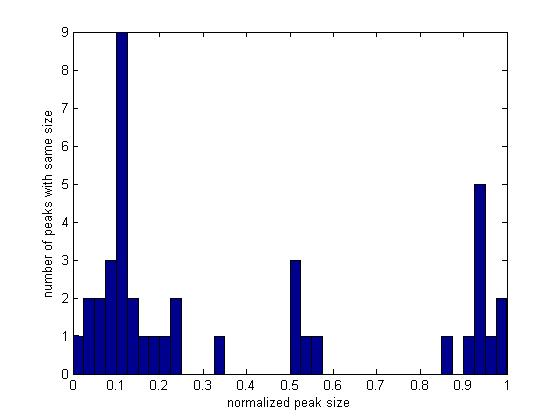
\includegraphics[width=0.7\textwidth]{staffHorizontalHist.jpg}
		\caption{Frequency of the normalized staff peak values \label{fig:staffHorizontalHist}}
\end{figure}

Extracting locations of the peaks higher than threshold from the projection returns the positions (row numbers) of all staff line centers. 


To detect the correct threshold is not always straight forward. In figure~\ref{fig:staffHard}(a) it is easy for humans to detect the peaks caused by staff lines. But the alogirhtm determines the threshold with figure~\ref{fig:staffHard}(b) and there it is not as clear, which values belong to the staff lines. Due to this there are sometimes to many lines marked as staff lines, see figure~\ref{fig:staffHard}(c). Especially the music title or text to sing delivers false positives. To detect the false positives are several steps necessary. First k-means  algorithm is applied to sort the lines into different clusters. Each cluster represents a staff system and has to consist out of exact 5 lines. The number of seeds for k-means is determined by number of lines found modulo 5. The seed positions are marked in gray in figure~\ref{fig:staffHard}(d). Then k-means defines the clusters for staff lines, see figure~\ref{fig:staffHard}(e).
Now the false positives can be easily detected by the distance of the lines per each cluster. After throwing away the outliers the result is the detected staff lines, see figure~\ref{fig:staffHard}(f).



\begin{figure}[htbp]
	\centering
    
  \begin{subfigure}[b]{0.48\textwidth}
        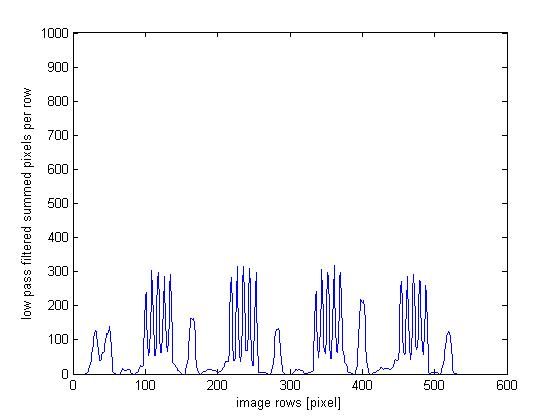
\includegraphics[width=\textwidth]{staff_textLinesHorizontalFiltered.jpg}
        \caption{Horizontal projection filtered for finding staff lines}
  \end{subfigure}
  \begin{subfigure}[b]{0.48\textwidth}
        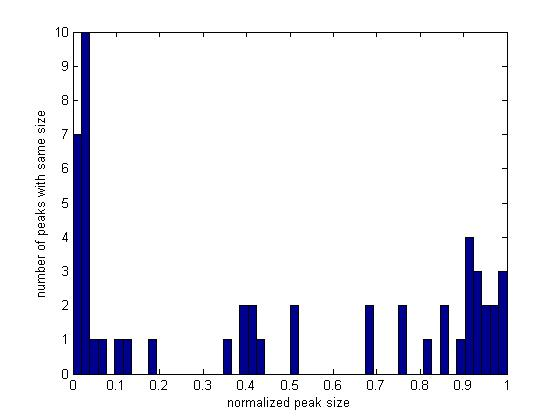
\includegraphics[width=\textwidth]{staff_textLinesHorizontalFilteredHist.jpg}
        \caption{Frequency of the normalized staff peak values}
  \end{subfigure}
    \begin{subfigure}[b]{0.48\textwidth}
        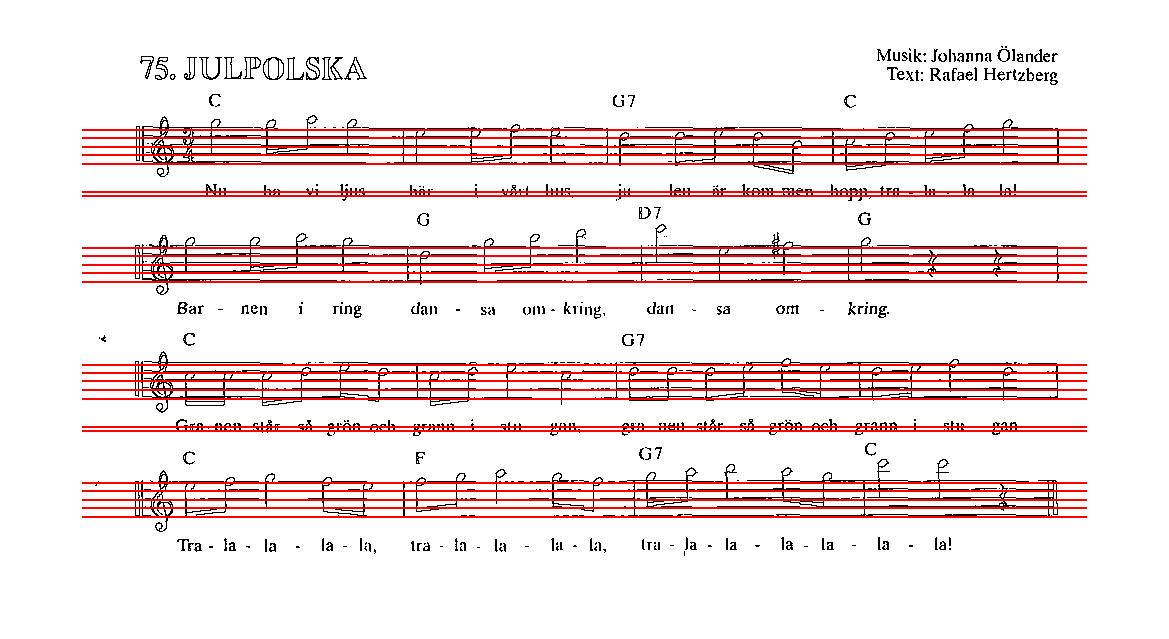
\includegraphics[width=\textwidth]{staff_textLines_staffLines.jpg}
        \caption{Detected lines (red) with high probability to be a staff line}
  \end{subfigure}
  \begin{subfigure}[b]{0.48\textwidth}
        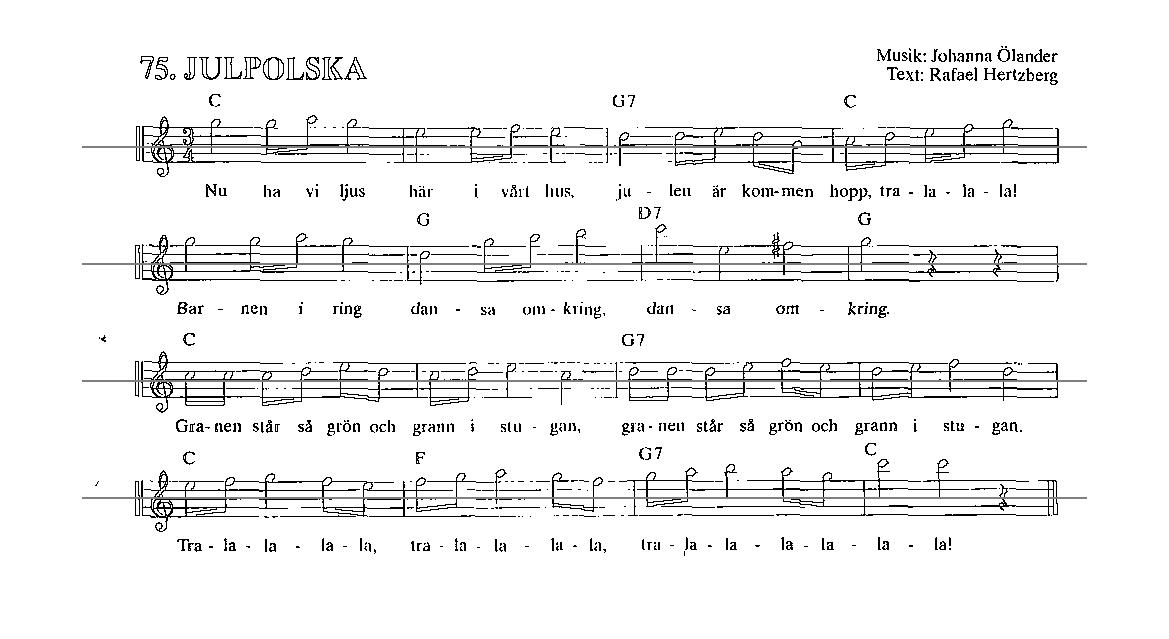
\includegraphics[width=\textwidth]{staff_textLines_seeds.jpg}
        \caption{Seed positions (gray) for k-means algorithm based on detected staff lines}
  \end{subfigure}
  \begin{subfigure}[b]{0.48\textwidth}
        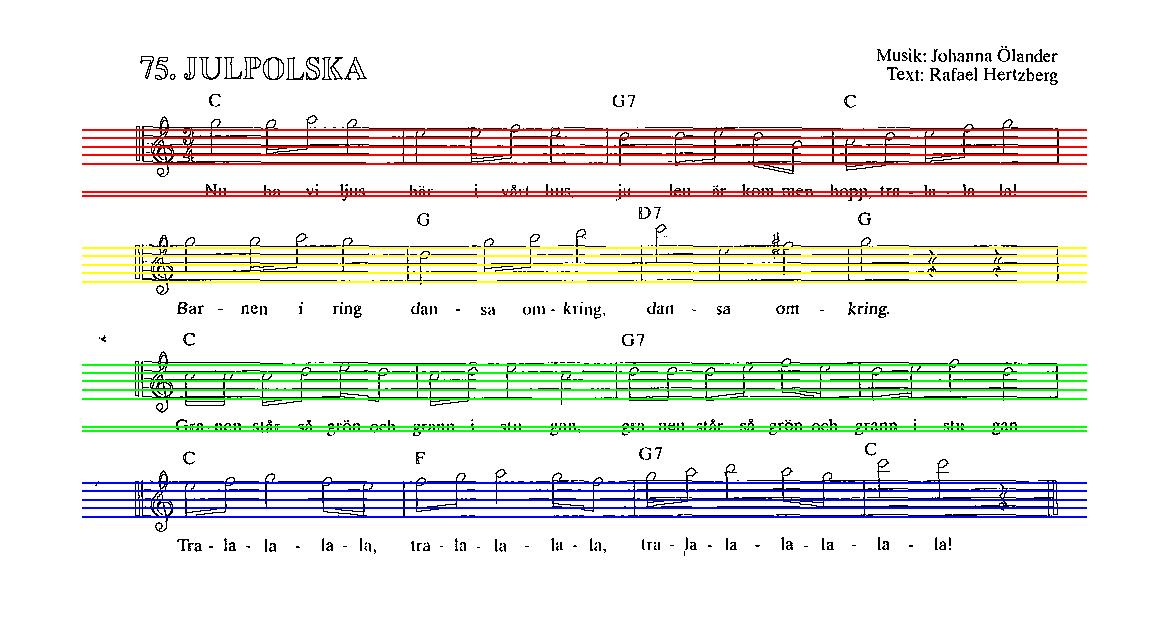
\includegraphics[width=\textwidth]{staff_textLines_cluster1.jpg}
        \caption{Detected staff lines in clusters, each color shows one cluster}
  \end{subfigure}
  \begin{subfigure}[b]{0.48\textwidth}
        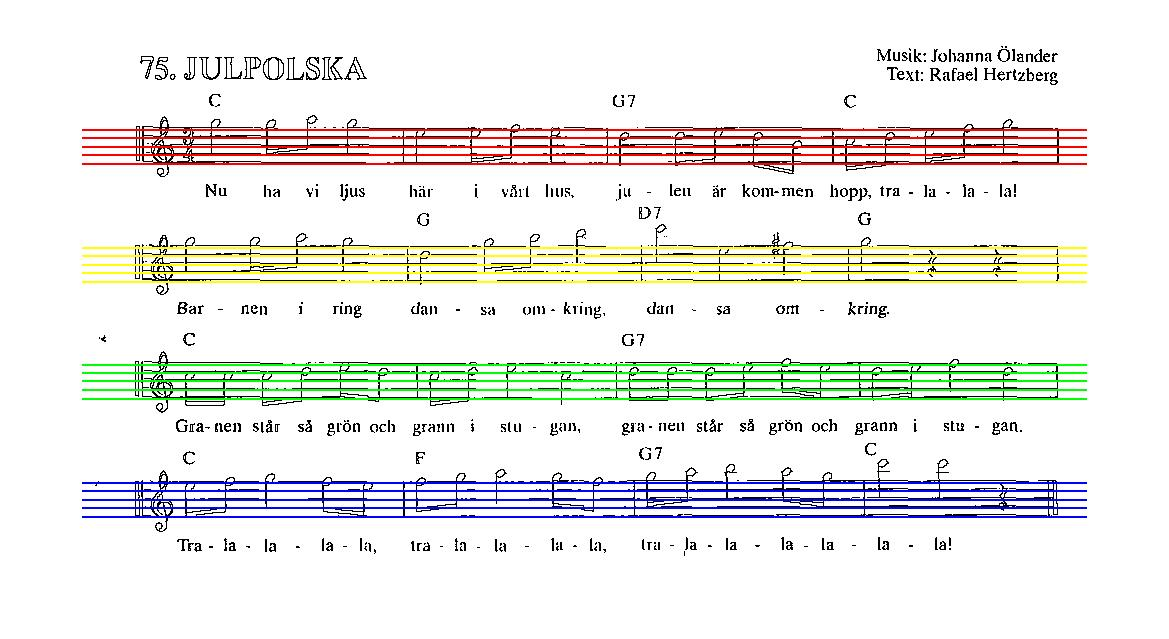
\includegraphics[width=\textwidth]{staff_textLines_cluster2.jpg}
        \caption{Detected staff lines in clusters after removing outliers}
  \end{subfigure}
	\caption{Detect staff lines with false positives due to text lines}
	\label{fig:staffHard}
\end{figure}


With the knowledge of the staff system a big step in note detection is done. Now it is possible to determine \textit{staffSpace} and \textit{staffHeight}. Those values are needed in nearly every following step. 




%#######################################
\subsection{Detect cut borders}
%#######################################

Only the part with notes is interesting for further steps. So everything else can be cutted away. This means for example title or background like table.
The picture has 4 edges and this delivers 4 sides where a axis aligned cut is possible. 


The rule to find the cutpositions above and below the staff system is quite easy. As the beams of the notes could go above and below their staff space, it is not possible to cut directly before the first and after the last staff system. Instead an offset has to be added. This offset is a little bit bigger than one staff system.
So this offset is added to the end of the last staff system and substracted from the beginning of the first staff system to define the upper and the lower cut.

Defining the left cut border is a bit more complicated. 
As given in the task description  Treble Clef (G-clef) is always assumed. Therefore the G-clef should be removed. Otherwise it will be the reason for false positives in note detection later on. But how to detect the G-clef? In the vertical projection of the image the G-clef can be identified as highest peak in the left quad, see figure~\ref{fig:leftCut}. Due to this reason the left cut is set to be at the position of the first minima after the first peak, because this is the position, where the G-clef ends. A cut on the right side was not necessary for this implementation.

Now the image is normalized and well prepared for the following steps. Figure~\ref{fig:normalized} shows the image from figure~\ref{fig:leftCut} as normalized version.

\begin{figure}[htbp]
	\centering
    
  \begin{subfigure}[b]{0.81\textwidth}
        \hspace*{3mm}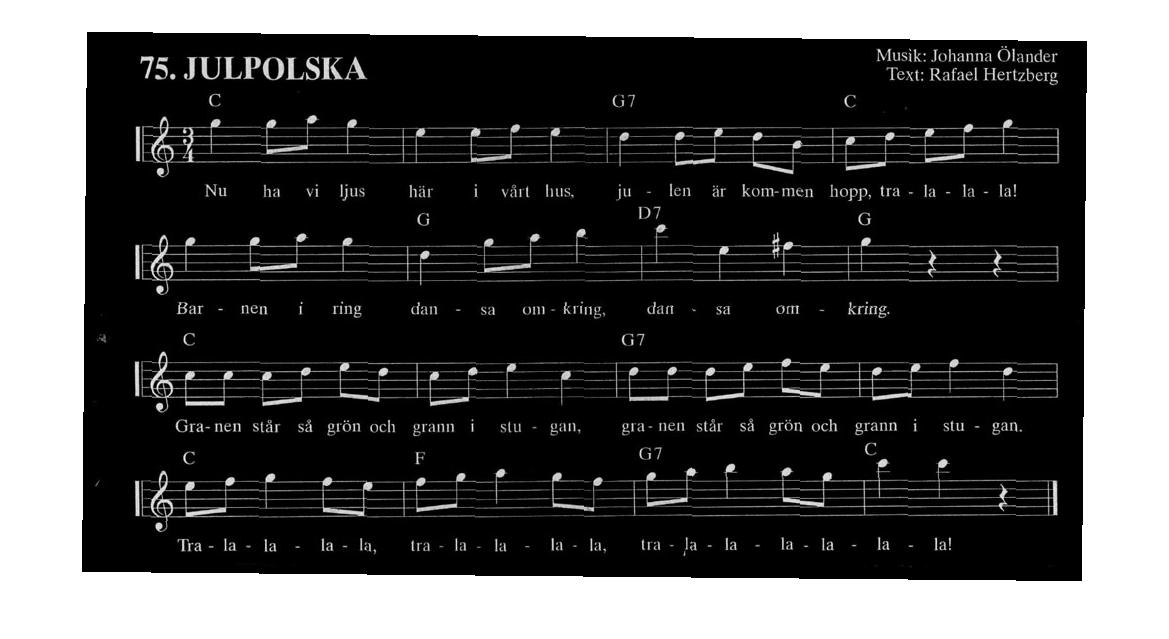
\includegraphics[width=\textwidth]{detectCut_lied.jpg}
        \caption{Binarized, complemented, rotated image}
  \end{subfigure}
  
  \begin{subfigure}[b]{0.9\textwidth}
        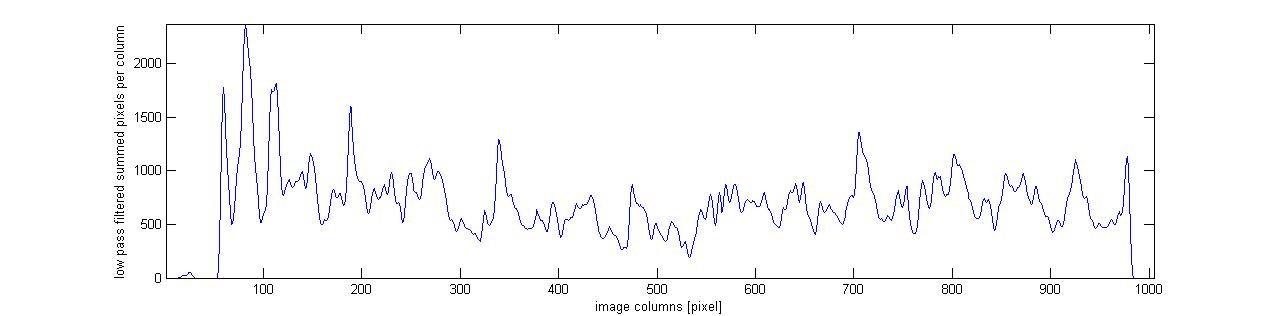
\includegraphics[width=\textwidth]{detectCut_plot.jpg}
        \caption{Vertical filtered projection (of counting white pixels)}
  \end{subfigure}
  	\caption{Image and vertical projection to define left cut border}
	\label{fig:leftCut}
  \end{figure}


\begin{figure}[Htbp]
    \centering
    % links, unten rechts oben
		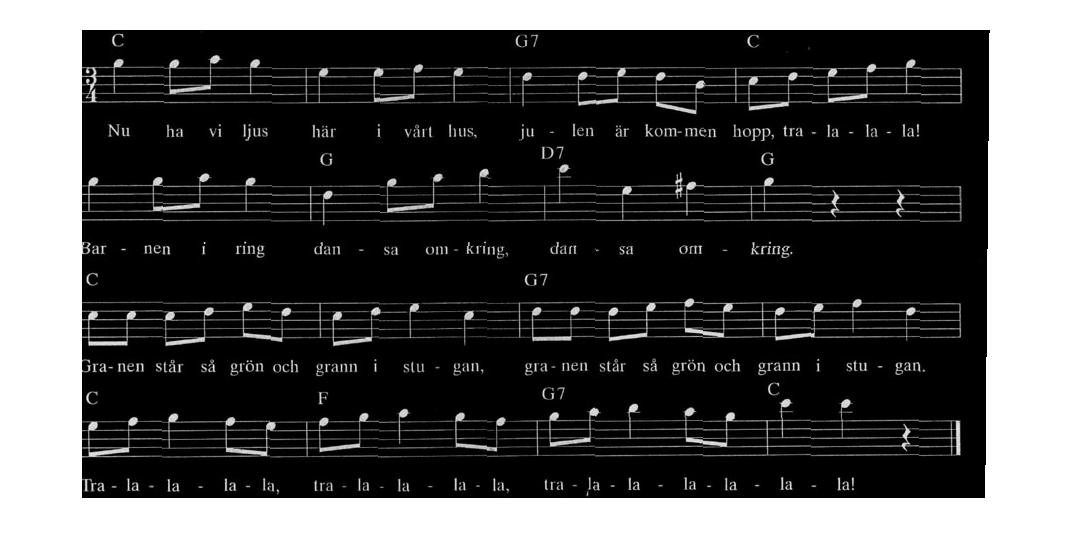
\includegraphics[width=0.65\textwidth]{normalized.jpg}
		\caption{Example for normalized image \label{fig:normalized}}
\end{figure}


%##############################################################################
%##############################################################################
\section{Detect Notes}
%##############################################################################
%##############################################################################
After the normalization process, the image is assumed to be a note sheet containting less unnecessary information than the original sheet. The normalized image is the image source used for detection. In the following chapters describes first the process of getting different image variations that provides different informations. After extracting these informations and combine them, it is possible to determine the note values and their pitch. Finally out of this data the string is derived.  
%#######################################
\subsection{Create Image Variations}
%#######################################
A set of different images of the sheet music is derived through various morphological operations. This set includes images with:

\begin{itemize}
\item note heads only
\item no staff lines 
\item no staff lines, strenghtend all remaining areas
\end{itemize}

\begin{figure}[htbp]
	\centering
    
  \begin{subfigure}[b]{0.7\textwidth}
        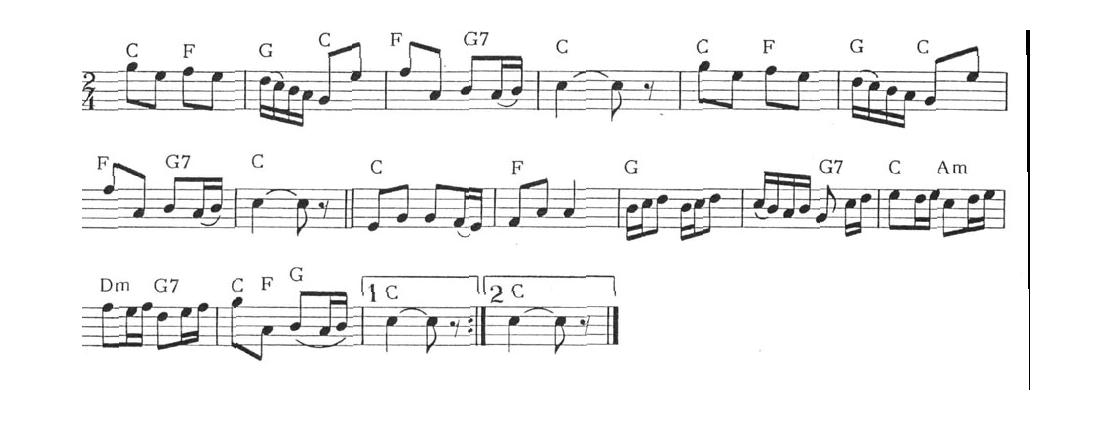
\includegraphics[width=\textwidth]{iv_orig.jpg}
        \caption{Original image, rotated and cutted}
  \end{subfigure}
  \begin{subfigure}[b]{0.7\textwidth}
        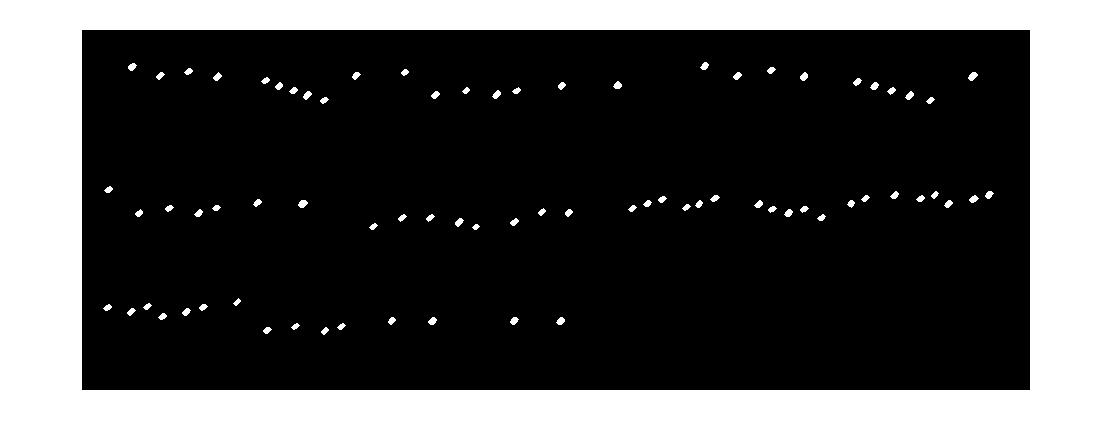
\includegraphics[width=\textwidth]{iv_noteHeads.jpg}
        \caption{Focused on note heads}
  \end{subfigure}
    \begin{subfigure}[b]{0.7\textwidth}
        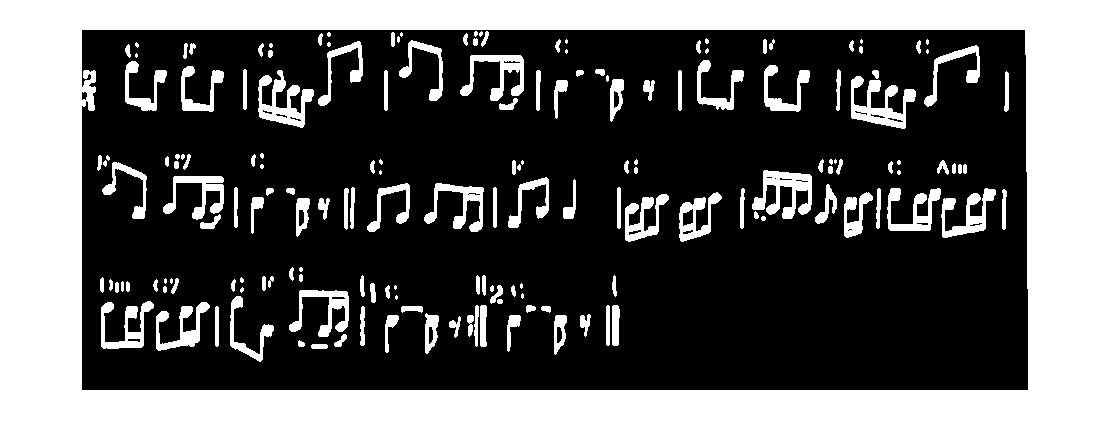
\includegraphics[width=\textwidth]{iv_boxes.jpg}
        \caption{Removed staff and strengthened areas}
  \end{subfigure}
    \begin{subfigure}[b]{0.7\textwidth}
        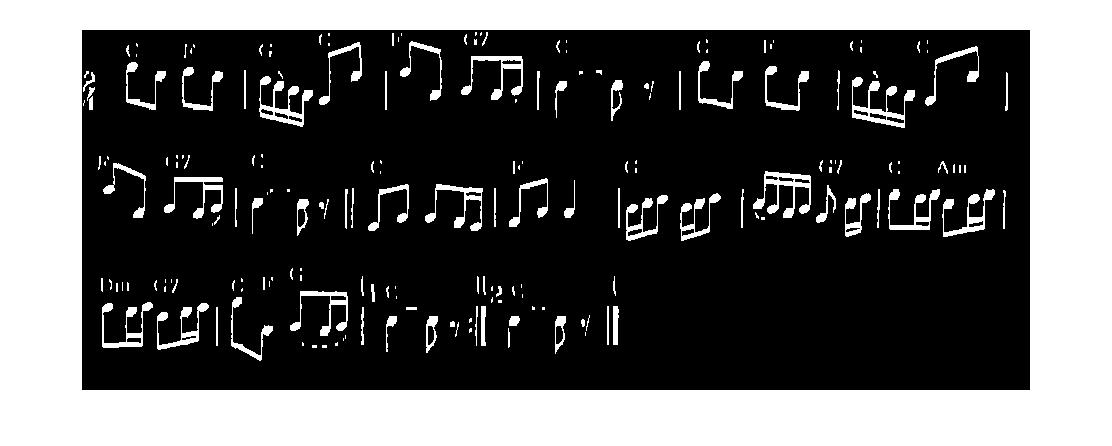
\includegraphics[width=\textwidth]{iv_remStaff.jpg}
        \caption{Removed staff}
  \end{subfigure}
  \begin{subfigure}[b]{0.7\textwidth}
        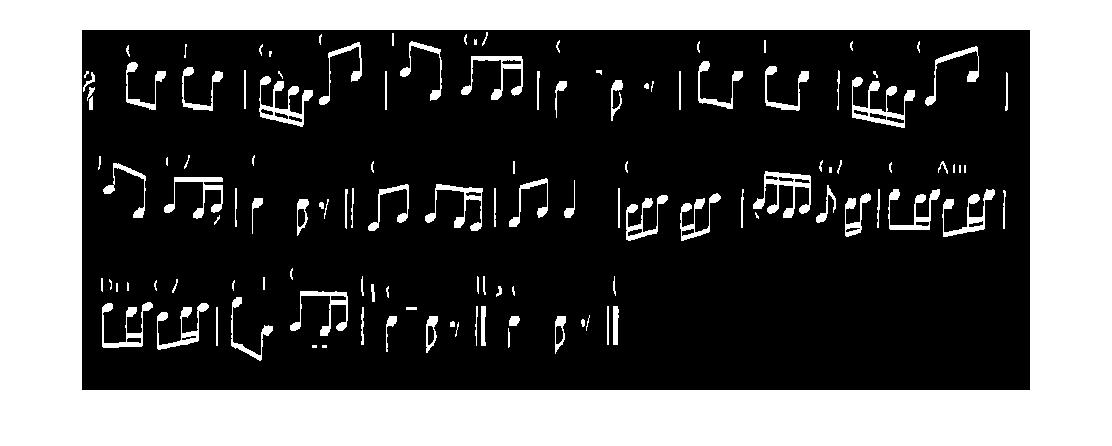
\includegraphics[width=\textwidth]{iv_remStaff_afterDefiningAreaSize.jpg}
        \caption{Removed staff and noise}
  \end{subfigure}
	\caption{Different image variations}
	\label{fig:variations}
\end{figure}





\paragraph{Note heads only}
To remove everything except note heads, the normalized image, compare  figure~\ref{fig:variations}(a), is opened with a disk element. The size of the disk element depends on the \textit{staffSpace}, see  figure~\ref{fig:variations}(b). 


\paragraph{No staff lines, strengthened all remaining areas}
The main goal with this variation is to get all the connected areas like quavers connected with a note beam. To get the best result, the normalized image can not be used directly. Instead the rotation and cut algorithms from the normalizing step are applied to the original image. Then this gray value image is opened with a vertical line structuring element to remove the staff lines. This result is then binarized after enhancing the vertical information and opened once more with the same element. Finally, the image is dilated with a cross shaped structuring element. This step ensures that note heads barely connected to their steam get connected, see figure~\ref{fig:variations}(c).  

\paragraph{No staff lines}
Next, in order to get an image with no staff lines and only rare information, the normalized image is opened twice with a vertical line structuring element. This results in  figure~\ref{fig:variations}(d). As this image contains to much noise, an additional operation is needed. The modified images gets opened again, ensuring that all the areas remaining have at least a size of 2 times \textit{staffSpace} pixels, compare  figure~\ref{fig:variations}(e).



%#######################################
\subsection{Detect note heads}
%#######################################
In this step the note head focused image variation is used. This image contains the note heads only. To locate the density positions of the note heads, the matlab functions bwlabel followed by regionsprops with the centroid property are used. To give the notes the correct order for building the result string the notes get sorted by their staff membership and x position. 


%#######################################
\subsection{Detect connected areas}
%#######################################
After detection of all connected areas in the image with strengthened objects, the areas get checked for their size. Each note including its steam is expected to be at least 3 times \textit{staffSpace} high. All areas that do not reach this minimum hight gets deleted. The remaining area boundung boxes are stored for the note value detection. In case of the note being a quaver, even the note beams are inside this axis aligned boxes.



%#######################################
\subsection{Detect note values}
%#######################################
This keyfunction combines a lot of previous calculated informations to finally detect the note values. 

To show how the algorithm works, the processing for 5 notes will be explained in this chapter. Figure~\ref{fig:boundingBoxes} shows the notes that are explored.

\begin{figure}[Htbp]
    \centering
		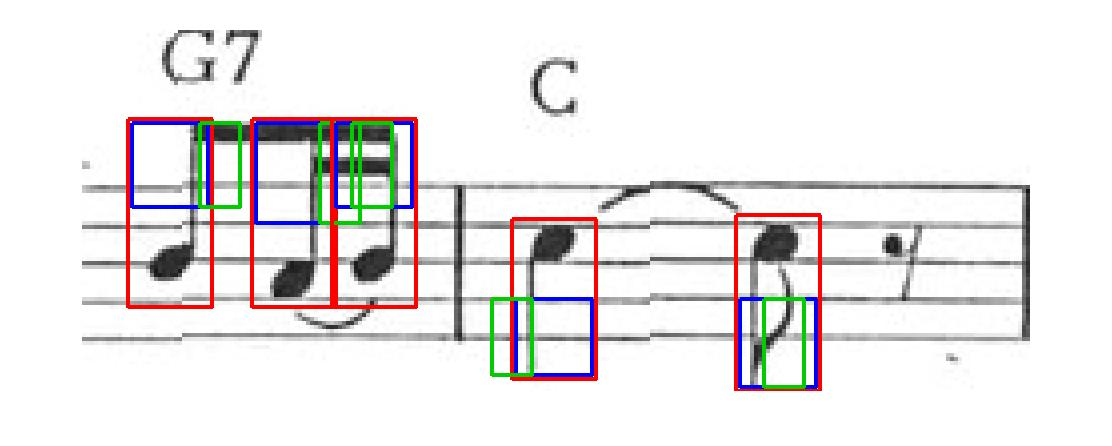
\includegraphics[width=0.65\textwidth]{boundingBoxes.jpg}
		\caption{Bounding boxes with color coding, see next figures \label{fig:boundingBoxes}}
\end{figure}


The general algorithm is for every note the same. For each note head position make a look up in the axis aligned boxes. If the note head position belongs to a real note, there is a box, which contains this position. Otherwise the note head is with a high probability not a note head. Continue with those note heads that were in a box. 

For every note take the found containing box. This boxes represents the note and its surrounding. To be able to get the note and its surrounding information the image without staff information is accessed and the information inside the box is extracted. 

Next all these image parts are normalized. This normalization means that all the notes can be handled in the same way. Therefore all image information above the center of the notehead is flipped downwards. This results in an image like figure~\ref{fig:noteValues1}(a). 

The note head is now cutted away so that it doesn't inlfuence the analysing of the beams, see figure~\ref{fig:noteValues1}(b). On this image a horizontal projections is made, see figure~\ref{fig:noteValues1}(c). This projection shows the beam position by it's maximum value. 

In general, music note values are defined by the side regarding the steam that has the most information. For example in figure~\ref{fig:noteValues2}(b) and (c) the side that determines the note value is the right side. If there is no further information except the steam itself, the note is classified as a crotch, see figure~\ref{fig:noteValues4}(c).

Once the side of the important information is known, only this side is further analysed. Therefore a new extraction is made. This new extraction has a fixed boxsize and is positioned next to the steam on the important side, see figure~\ref{fig:noteValues1}(d).

From this image a horizontal projection is made, see figure~\ref{fig:noteValues1}(e). To reduce noise again a low pass filter is applied, see figure~\ref{fig:noteValues1}(e). By counting the number of peaks in this last image it is possible, to define the value of the note. One beam means a quavers and more than one beam is not considered in this application. 

The following figures show the extracted images and plots for different cases.

\begin{figure}[htbp]
	\centering
    
  \begin{subfigure}[t]{0.1\textwidth}
        
\includegraphics[width=\textwidth]{1a.jpg}
        \caption{red}
  \end{subfigure}
  \begin{subfigure}[t]{0.1\textwidth}
        
\includegraphics[width=\textwidth]{1b.jpg}
        \caption{blue}
  \end{subfigure}
    \begin{subfigure}[c]{0.4\textwidth}
        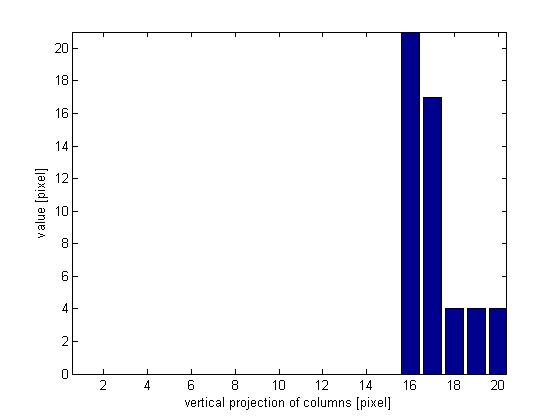
\includegraphics[width=\textwidth]{1c.jpg}
        \caption{vertical projection of columns}
  \end{subfigure}
  
  \begin{subfigure}[c]{0.1\textwidth}
        
\includegraphics[width=\textwidth]{1d.jpg}
        \caption{green}
  \end{subfigure}
  \begin{subfigure}[c]{0.4\textwidth}
        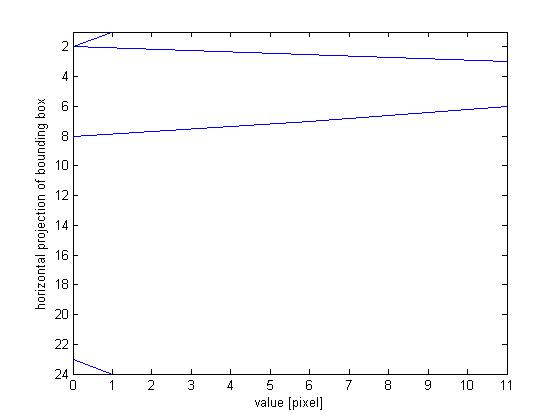
\includegraphics[width=\textwidth]{1e.jpg}
        \caption{horizontal projection of rows}
  \end{subfigure}
  \begin{subfigure}[c]{0.4\textwidth}
        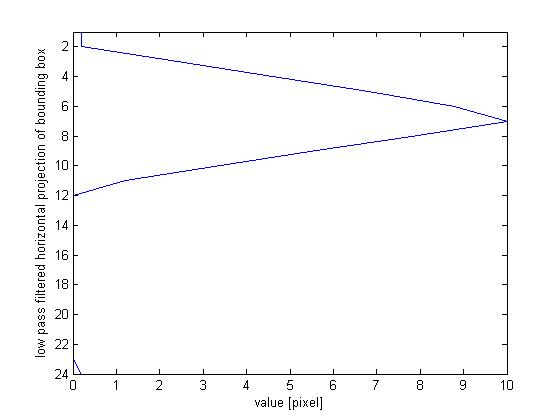
\includegraphics[width=\textwidth]{1f.jpg}
        \caption{filtered horizontal projection of rows}
  \end{subfigure}
	\caption{Processing of note detection first note}
	\label{fig:noteValues1}
\end{figure}

\begin{figure}[htbp]
	\centering
  \begin{subfigure}[t]{0.1\textwidth}
        
\includegraphics[width=\textwidth]{2a.jpg}
        \caption{red}
  \end{subfigure}
  \begin{subfigure}[t]{0.1\textwidth}
        
\includegraphics[width=\textwidth]{2b.jpg}
        \caption{blue}
  \end{subfigure}
    \begin{subfigure}[c]{0.4\textwidth}
        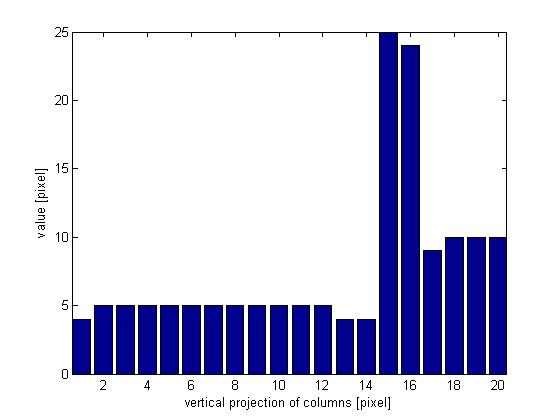
\includegraphics[width=\textwidth]{2c.jpg}
        \caption{vertical projection of columns}
  \end{subfigure}
  
  \begin{subfigure}[c]{0.1\textwidth}
        
\includegraphics[width=\textwidth]{2d.jpg}
        \caption{green}
  \end{subfigure}
  \begin{subfigure}[c]{0.4\textwidth}
        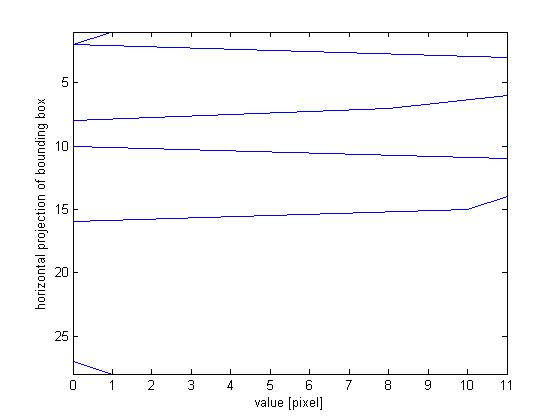
\includegraphics[width=\textwidth]{2e.jpg}
        \caption{horizontal projection of rows}
  \end{subfigure}
  \begin{subfigure}[c]{0.4\textwidth}
        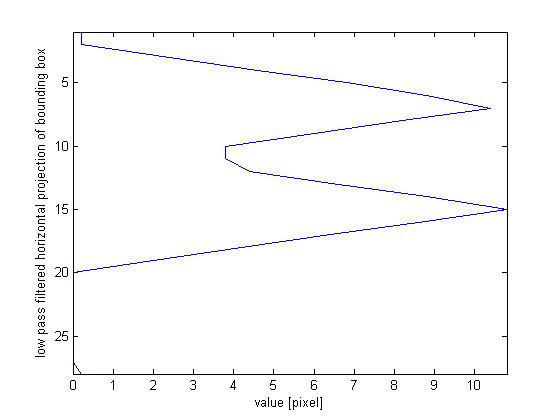
\includegraphics[width=\textwidth]{2f.jpg}
        \caption{filtered horizontal projection of rows}
  \end{subfigure}
	\caption{Processing of note detection second note}
	\label{fig:noteValues2}
\end{figure}

\begin{figure}
\centering
\begin{subfigure}[t]{0.1\textwidth}
        
\includegraphics[width=\textwidth]{3a.jpg}
        \caption{red}
  \end{subfigure}
  \begin{subfigure}[t]{0.1\textwidth}
        
\includegraphics[width=\textwidth]{3b.jpg}
        \caption{blue}
  \end{subfigure}
    \begin{subfigure}[c]{0.4\textwidth}
        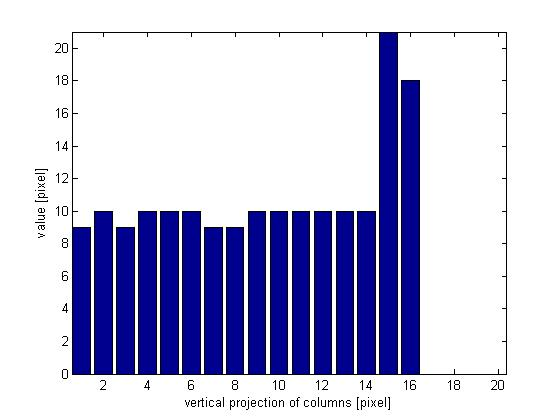
\includegraphics[width=\textwidth]{3c.jpg}
        \caption{vertical projection of columns}
  \end{subfigure}
  
  \begin{subfigure}[c]{0.1\textwidth}
        
\includegraphics[width=\textwidth]{3d.jpg}
        \caption{green}
  \end{subfigure}
  \begin{subfigure}[c]{0.4\textwidth}
        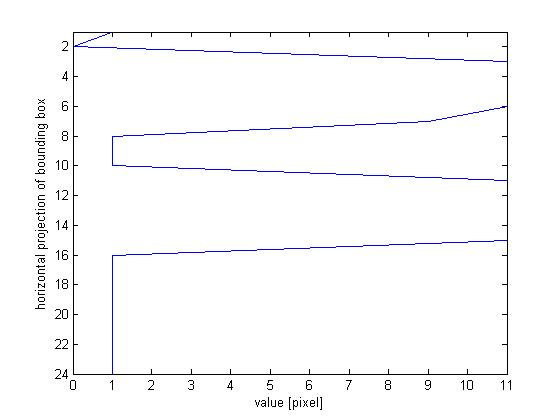
\includegraphics[width=\textwidth]{3e.jpg}
        \caption{horizontal projection of rows}
  \end{subfigure}
  \begin{subfigure}[c]{0.4\textwidth}
        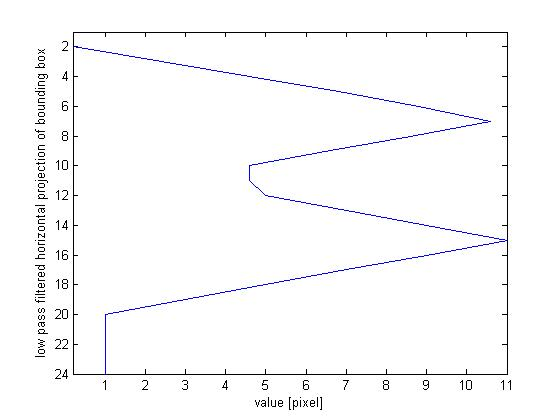
\includegraphics[width=\textwidth]{3f.jpg}
        \caption{filtered horizontal projection of rows}
  \end{subfigure}
	\caption{Processing of note detection third note}
	\label{fig:noteValues3}
\end{figure}


\begin{figure}
\centering
\begin{subfigure}[t]{0.1\textwidth}
        
\includegraphics[width=\textwidth]{4a.jpg}
        \caption{red}
  \end{subfigure}
  \begin{subfigure}[t]{0.1\textwidth}
        
\includegraphics[width=\textwidth]{4b.jpg}
        \caption{blue}
  \end{subfigure}
    \begin{subfigure}[c]{0.4\textwidth}
        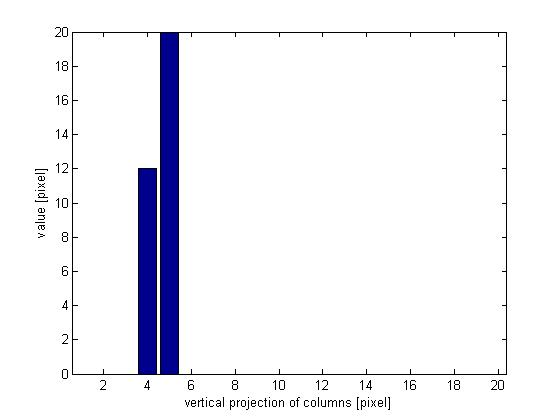
\includegraphics[width=\textwidth]{4c.jpg}
        \caption{vertical projection of columns}
  \end{subfigure}
	\caption{Processing of note detection fourth note}
	\label{fig:noteValues4}
\end{figure}

\begin{figure}
\centering
\begin{subfigure}[t]{0.1\textwidth}
        
\includegraphics[width=\textwidth]{5a.jpg}
        \caption{red}
  \end{subfigure}
  \begin{subfigure}[t]{0.1\textwidth}
        
\includegraphics[width=\textwidth]{5b.jpg}
        \caption{blue}
  \end{subfigure}
    \begin{subfigure}[c]{0.4\textwidth}
        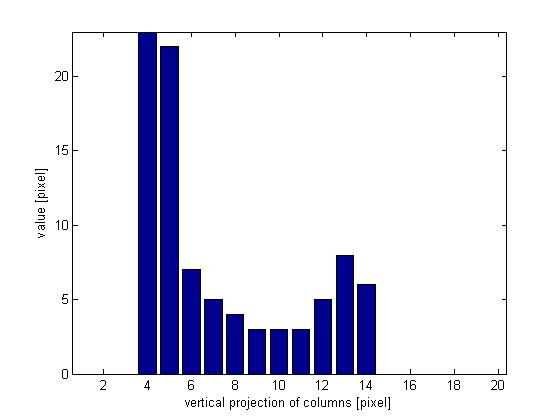
\includegraphics[width=\textwidth]{5c.jpg}
        \caption{vertical projection of columns}
  \end{subfigure}
  
  \begin{subfigure}[c]{0.1\textwidth}
        
\includegraphics[width=\textwidth]{5d.jpg}
        \caption{green}
  \end{subfigure}
  \begin{subfigure}[c]{0.4\textwidth}
        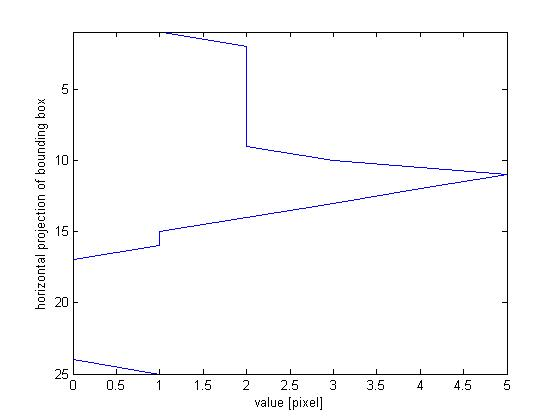
\includegraphics[width=\textwidth]{5e.jpg}
        \caption{horizontal projection of rows}
  \end{subfigure}
  \begin{subfigure}[c]{0.4\textwidth}
        \includegraphics[width=\textwidth]{5f.jpg}
        \caption{filtered horizontal projection of rows}
  \end{subfigure}
	\caption{Processing of note detection fifth note}
	\label{fig:noteValues5}
\end{figure}


%#######################################
\subsection{Build string and draw}
%#######################################
Finally all of the information is evaluated to generate the string to give back. 

The output should follow the following convention: (see even figure~\ref{fig:outputString})

\begin{itemize}
\item Uppercase letters for crotches
\item Lowercase letters for quavers
\item Numbers from 1 to 4 indicating the pitch of each individual note
\item Multiple notes:
Register each note separately, from top to bottom
\item Line break (new staff) shall be encoded with the character n
\end{itemize}

%\begin{figure}[th]
    %\centering
		%\includegraphics[width=0.7\textwidth]{outputString.png}
		%\caption[The output string] { The output string should follow the following convention: uppercase letters for crotches and lowercase letters for quavers \label{fig:outputString}}
%\end{figure}

With the knowledge of note value and the absolut positon of the note head in the staff system the note pitch can be detected straight forward. 

To have not only the string feedback this application is able to print the detected notes by color coding on the images.
This way supplies a much faster way to manually identify correct and incorrect detections. Figure~\ref{fig:finalImage} shows one of those images. The images for all test images can be found in the appendix. 

\begin{figure}[th]
    \centering
		\includegraphics[width=0.9\textwidth]{im1s_compare.jpg}
		\caption[Recognized notes drawn on original, cutted image]{Recognoized notes drawn on original, cutted image. Color coding: blue-not considered, green-quavers,  yellow-crotches \label{fig:finalImage}}
\end{figure}



%##############################################################################
%##############################################################################
\section{Alternative Approaches}
%##############################################################################
%##############################################################################

There are different other approaches to determine notes. Especially when all notes and symboles have to be recognized.

One other possibilty is the application of template matching. But then the \textit{staffSize} becomes more important. For every detection different templates have to be used regarding the \textit{staffSize}.
In \cite{Mcpherson_2002_IntrFeedIntoAn} an approach is described to adapt the patterns during matching time, to be more robust in symbol detection. 


%##############################################################################
%##############################################################################
\section{Conclusion, Result and Analysis}
%##############################################################################
%##############################################################################

In this report the implementation of our OMR software is described. With a lot of examples the functionality is explained and the results for the test images are availabe in the appendix. 

The achieved software works very well for scanned image as input. There are some minor mistakes, like detecting notes out of a break. This could be solved by using template matching. The template matching at that position would show, that the object is not a note. 

If the quality of the scanned notes is poor and parts of the notes are missing, then the recognition fails. This is a general problem for optical recognition software. One idea how to solve this problem is the use of more intelligent algorithms. For example between 3 notes with beams, there is a high probability that there is a fourth note inside, when there is enough space, see fourth staff system in figure~\ref{fig:allemande}. This post processing can be very complex.

The step detect borders, described in chapter 2.4 is made for convenience purpose only. We make use of the preconditions allowing us to throw away unnecessary information, making the rest of the analysis a lot easier. The advantage of this approach is obvious: we do not get the false positives from the dot of the G clef, instead though there is a small chance that we do loose correct notes if they happen to be too close. This works really well for us, but it not suited for general music recognition.

The preprocessing works only rudimentary. There are possibilities to extend the preprocessing with the written stages. 

All in all within this project work a software was developed which works realy well for the given images. Nevertheless software can always be improved.


\newpage
%#######################################
\bibliographystyle{plaindinBirgit}
%\bibstyle{plain}
\phantomsection
\addcontentsline{toc}{section}{References}
\bibliography{bibliography}
%\printbibliography
%#######################################	
	
	\newpage
\section*{Appendix}
\addcontentsline{toc}{section}{Appendix}

On the following sides are the results for the scanned test images.

\begin{sidewaysfigure}[Htb]
    \centering
		\includegraphics[width=\textwidth]{im1s_compare.jpg}
		\caption[Dance]{Dance  'g3e3f3e3g2e3f3a2b2C3c3g3e3f3e3g2e3nf3a2b2C3c3e2g2g2f2a2A2d3d3g2e3c3nf3d3g3a2b2C3c3C3c3'}
\end{sidewaysfigure}

\begin{sidewaysfigure}[Htb]
    \centering
		\includegraphics[width=\textwidth]{im3s_compare.jpg}
		\caption[Julpolska]{Julpolska 'G3g3a3G3E3e3f3E3D3d3e3d3b2c3d3e3f3G3nG3g3a3G3D3g3a3B3C4E3F3G3n \newline c3c3c3d3e3d3c3d3E3C3d3d3d3e3f3e3d3e3F3D3ne3f3G3f3e3f3g3A3g3f3g3a3B3a3g3C4C4'}
\end{sidewaysfigure}

\begin{sidewaysfigure}[Htb]
    \centering
		\includegraphics[width=\textwidth]{im5s_compare.jpg}
		\caption[Allegro]{Allegro 'd3b2d3g3d3b2d3b2g2f2a2d2f2a2c3e3c3a2f2d2f2g2d2g2b2d3b2g3d3b2d3b2g2n \newline f2a2d2f2a2c3e3c3a2f2d2f2G2a2d3f3c3e3a2c3e3c3d3f3a2d3f3d3n \newline e3g3e3c3a2c3d3f3a3g3b3a3c3e3a2c3e3c3d3f3a2d3f3d3e3g3b3g3e3c3D3'}
\end{sidewaysfigure}

\begin{sidewaysfigure}[Htb]
    \centering
		\includegraphics[width=\textwidth]{im8s_compare.jpg}
		\caption[Pippi Langstrump]{Pippi Langstrump 'C2F2A2F2b2a2g2f2E2G2E2nC2F2A2F2b2a2g2f2E2G2C2E2n \newline A2a2a2A2A2B2a2a2G2g2g2G2f2f2E2F2nA2a2a2A2A2B2A2G2G2F2E2'}
\end{sidewaysfigure}

\begin{sidewaysfigure}[Htb]
    \centering
		\includegraphics[width=\textwidth]{im9s_compare.jpg}
		\caption[Bred dina vingar]{Bred dina vingar 'b2d3G3C4D3e3c3b2d3b3c4C4A3F3D3G2C3n\newline a3b3C4C4C4a3g3B3B3C4E3F3G3E3b2d3n \newline G3C4D3e3c3b2d3a3c4C4A3F3D3'}
\end{sidewaysfigure}

\begin{figure}[Htb]
    \centering
		\includegraphics[width=\textwidth]{im6s_compare.jpg}
		\caption[Titanic]{Titanic \newline
										 'G2g2G2G2F2G2F2G2n\newline
											G2g2G2G2F2G2n\newline 
											G2g2G2G2F2G2F2A2n\newline
											G2g2G2G2F2G2n\newline
											D2C3b2a2B2C3n\newline
											A2G2F2F2n\newline 
											D2C3b2a2B2C3n\newline 
											A2G2F2G2F2A2'}
\end{figure}

\begin{figure}[Htb]
    \centering
		\includegraphics[width=\textwidth]{im10s_compare.jpg}
		\caption[Naer det lider mot jul]{Naer det lider mot jul \newline
		'D3B3d3e3G3f3a3C4f3g3B3a3G3e3f3D3e3c3n\newline
		C3f3D3f3g3C4g3f3E3g3c4C4a3g3n\newline
		F3e3d3E3d3c3D3c3b2C3a2c3F3d3C3e3f3F3E3n\newline
		C3A3c3e3G3f3a3C4f3g3A3b3G3e3f3D3e3c3n\newline
		C3A3c3e3G3f3a3C4f3g3A3a3G3e3f3D3e3c3n\newline
		f3g3f3E3g3b3C4a3g3F3e3d3E3d3c3n \newline
		D3c3b2C3a2c3F3d3C3F3E3'}
\end{figure}

\begin{sidewaysfigure}[Htb]
    \centering
		\includegraphics[width=\textwidth]{im13s_compare.jpg}
		\caption[Allemande ]{Allemande 		'f3c3c3f3g3c3c3g3a3f3a3g3c3c3a3a3g3a3a3d3d3n\newline 		f3d3f3d3g3e3g3e3b3g3b3g3n 		e3c3f3a2b2f3c3e3F3g3c3c3f3g3c3d3a3a3d3d3a3n \newline
		g3c3C3g3f2d3g3f2e3f3d3f3d3n 
		b2g2C3C3B2' \label{fig:allemande}}
\end{sidewaysfigure}
	
	
\end{document}



